\section{Introdução}
Quando se trata de aprender a utilizar as funcionalidades avançadas de um editor de texto muito
antigo é preciso avançar um pequeno trecho por vez.
Para tecnologias antigas, existe na internet livremente todo tipo de dica,
todo tipo de vídeo, e até mesmo todo tipo de texto em pdf.
Mas um dos trabalhos deste documento é organizar para tornar mais orgânica a absorção.

O vim possui um tutorial, acessível pela linha de comando.
Basta escrever no seu prompt \vimcommand{\$ vimtutor} que o tutorial começa.
Assim como quase tudo na vida, você primeiro lê, depois tenta tomar alguma ação.
Pretendo seguir mais ou menos a mesma ordem do tutorial, mas com mais explicações.
Em alguns trechos teremos apenas a explicação e experimentar fica com você.

Para rodar o vimtutor, é preciso a versão do vim completa.
Portanto, o primeiro passo é instalar usando seu gerenciador de pacotes,
ou pesquisando na internet a forma de instalação para o seu sistema operacional.

\begin{figure}[!htb]
\centering
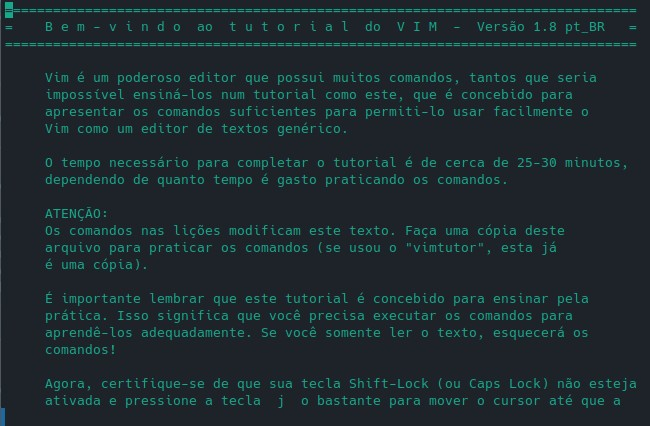
\includegraphics[scale=0.90]{introducao/vimtutor_enter_screen.jpg}
%\label{introducao_001}
\caption{O vimtutor é um bom ponto de partida.}
\end{figure}

Uma espécie de piada que aparece em certos meios é sobre não se saber sair do vim.
Podemos começar por aí.
Podemos iniciar o vim com ou sem um nome de arquivo especificado.
Digamos que entramos sem especificar usando o comando \vimcommand{\$ vi}.
Assim que se abre o vim entra-se no modo \emph{normal}.
Através de teclas de atalho podemos entrar em outros modos.
Existem poucas formas de intercambiar entre modos, sendo geralmente mais simples voltar
para o modo normal antes de seguir para um outro.
Para voltar para o modo normal, pressione \vimcommand{esc} repetidamente,
ou mesmo a combinação \vimcommand{Ctrl-C} para desativar o modo atual.
Se você não fez nenhuma alteração no texto que está na tela
basta apertar \vimcommand{:} para entrar no modo \emph{ex}.
O modo ex serve para inserção de comandos.
Inseriremos o comando \vimcommand{:quit}.

\begin{figure}[!htb]
\centering
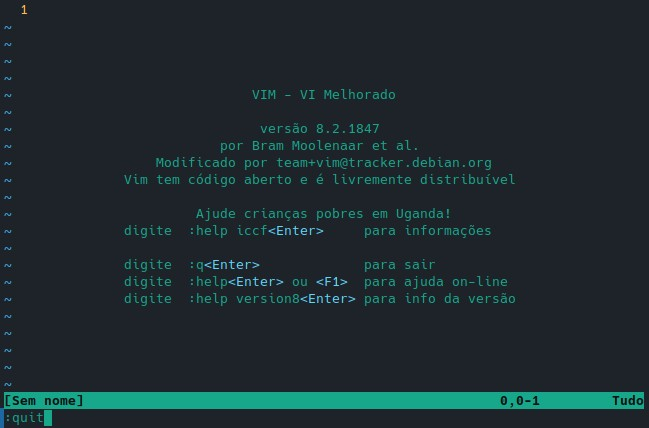
\includegraphics[scale=0.9]{introducao/comando_quit.jpg}
%\label{introducao_002}
\caption{Podemos sair do vim se quisermos.}
\end{figure}

É parte da cultura Unix criar comandos como abreviações de nomes maiores,
como cat que abrevia con\textbf{cat}enate.
Você pode sair usando apenas \vimcommand{:q}.

Novamente com o vim aberto, pode-se escolher salvar o arquivo, definindo o nome, com \vimcommand{:write [nome do arquivo]}.
Atenção. Os comandos diferenciam minúsculas de maiúsculas.
Caso você esteja no modo normal, pode apertar \vimcommand{ZZ} para salvar e sair. Um atalho para \vimcommand{:wq}.

\subsection{Um pouco de qualidade de vida}
O vim cru não é exatamente muito legal.
Mas podemos melhorar usando umas poucas configurações logo de cara.
A primeira é quebrar o modo de compatibilidade com o antigo VI, usando o comando \vimcommand{:set nocompatible},
ou de forma abreviada \vimcommand{:set nocp}.
Dessa forma, você terá informações extras na última linha da janela, que farão falta se não estiverem habilitadas.

A próxima melhoria em qualidade de vida é adicionar números de linha com o comando \vimcommand{:set number}, ou \vimcommand{:set nu}.
Como dependemos da contagem de linhas para alguns movimentos e alguns comandos, tê-la à vista é interessante.

Outra configuração interessante é \vimcommand{:set ruler}.
Ela mostra no canto inferior direito informações sobre a posição do cursor.

Usando \vimcommand{:set laststatus=2} você irá criar uma barra permanente que indicará o nome do arquivo,
se ele está salvo, e as informações que ruler trouxe.

Usando \vimcommand{:set wildmenu}, você poderá ter seus comandos completados ao pressionar \vimkeys{$<$TAB$>$}.
Outra maneira de verificar quais as opções disponíveis é utilizar \vimkeys{$<$CTRL D$>$}.
Caso você esteja procurando entre muitas opções e não tem paciência para ficar pressionando tab,
\vimkeys{$<$CTRL D$>$} pode salvar tempo.

A última configuração serve para visualizarmos os comandos executados, úteis para macros.
Essa opção só está disponível no vim completo, mas como eu não sei qual vim você irá utilizar...
Usando \vimcommand{:set showcmd} aparecerão à direita as teclas pressionadas.
Será útil apenas mais adiante, mas ajuda na qualidade de vida.

Abra o vim com \vimcommand{\$ vi ~/.vimrc} e escreva cada um desses comandos.
Usar o vim padrão sem eles é terrível.

Os comandeos são:
\begin{itemize}
    \item set nocompatible
    \item set ruler
    \item set number
    \item set showcmd
    \item set wildmenu
    \item set laststatus=2
\end{itemize}

\begin{figure}[!htb]
\centering
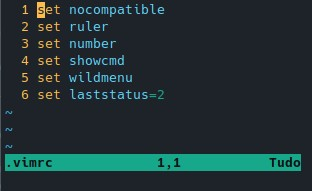
\includegraphics[scale=1.5]{introducao/vimrc_minimo.jpg}
%\label{introducao_003}
\caption{Crie este arquivo pelo seu próprio bem.}
\end{figure}

\subsection{Movimentação}
No modo normal fazemos as movimentações de cursor mais avançadas.
Dependendo da sua versão de vim, você pode usar as setas do teclado para se mover,
e pode realizar essa movimentação mesmo dentro do modo de inserção de texto.
Neste trecho do tutorial existe muito mais o que fazer do que mostrar,
então abra o seu vim e comece a testar.

Vamos ver o básico de movimentação:
\begin{itemize}
    \item \vimcommand{h} - Move para a esquerda.
    \item \vimcommand{j} - Move para baixo.
    \item \vimcommand{k} - Move para cima.
    \item \vimcommand{l} - Move para a direita.
\end{itemize}

\begin{figure}[!htb]
\centering
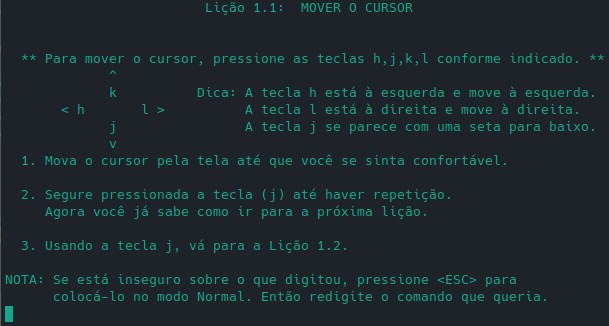
\includegraphics[scale=0.8]{introducao/movim_minimo.jpg}
%\label{introducao_004}
\caption{Movimentação básica.}
\end{figure}


\subsubsection{Lógica Número-Ação-Movimento}
Em muitos casos podemos pedir que o vim interprete nossos comandos com um multiplicador.
Isso significa que, ao invés de pressionar \vimcommand{l} para andar para a direita 10 vezes,
podemos escrever \vimcommand{10l}, e a mágica acontece.
Essa lógica vai nos acompanhar, e inclusive vai ficar mais rebuscada à medida que começamos a misturar conhecimentos.
Futuramente colocaremos a ação na brincadeira, completando assim o número-ação-movimento.

% -------Movimentação por palavras -----------------

Além de movimentação em relação aos caracteres, podemos nos movimentar em relação às palavras.
Isso significa que podemos usar o equivalente a CTRL-direita ou CTRL-esquerda que temos em editores como o MS Word.
Para pular palavras a frente temos duas opções.
Pressionar \vimcommand{w} pula para a primeira letra da próxima palavra.
Para pular para a última letra da palavra mais próxima, \vimcommand{e}.
Usar estes comandos com letras maiúsculas irá ignorar pontuações, assim, apenas considerando espaços vazios.
Geralmente existem diferenças maiores entre comandos de letras maiúsculas e minúsculas.

Para voltar, \vimcommand{b}, que pula para a primeira letra da palavra anterior.
Para pular para a última letra da palavra anterior, \vimcommand{ge}.
Mais tarde vamos aprender que a tecla \vimcommand{g} é uma tecla separada para comandos sem muita lógica associada.
Talvez seja isso mesmo, genérico, geral.

Por fim, para simplificar: \vimcommand{w} vai pra próxima word. \vimcommand{b} faz um "backword".
Sempre bom encontrar maneiras de lembrar das palavras chave, mnemônicos ajudam.

% -------Movimentação na linha  -----------------

Podemos pular também para o começo ou fim da linha de texto.
Para pular para o primeiro caractere da linha, pressionamos \vimcommand{0}.
Para o último caractere, \vimcommand{\$}.
Quando desenvolvendo programas, existe a necessidade de se pular para o primeiro caractere não nulo.
Para fazer essa ação, podemos usar o comando \vimcommand{\^}.

Já falamos de palavras, de caracteres, e fomos para começo e fim da linha.
Podemos fazer o cursor viajar até um certo caractere.
Para essa ação escrevemos \vimcommand{t\_}, que significa "até o caractere \_".
A mesma ação, mas para trás, é usar \vimcommand{f\_}.
E, novamente, para ficar mais fácil de lembrar, "unTil \_".
E para a ação reversa, "find \_".

O uso de T e F fica a seu cargo de compreender.
Afinal de contas, não é porque não ensinei que você não vai aprender.

% -------Movimentação entre parênteses -----------------

Novamente, existe a funcionalidade de pular entre uma ponta ou outra de um pedaço de
texto que esteja dentro de parênteses, chaves ou colchetes.
Quando se está programando, isso faz muito sentido, já que existem grandes trechos de
códigos que podem estar enclausurados nestes caracteres.
A ação é \vimcommand{\%}.

% -------Movimentação entre parágrafos -----------------

Voltando ao texto normal, podemos pular parágrafos.
Estamos ficando bons em pular grandes trechos.
Para pular, \vimcommand{\{} e \vimcommand{\}}. Experimente.

% -------Movimentação pelo histórico de saltos -----------------

Sempre que fazemos um grande salto no vim deixamos um rastro na memória.
Podemos abusar disso para pular de forma eficiente.
Para voltar no histórico de pulos, \vimcommand{CTRL-O} para voltar.
Para avançar usamos \vimcommand{CTRL-I}.
Futuramente podemos verificar como pular entre palavras específicas.
Além disso, podemos pular entre palavras que não estão no mesmo arquivo aberto.

% -------Movimentação para começo/fim do arquivo -----------------
Para finalizar.
Podemos fazer mais dois tipos de salto, um para as pontas do arquivo, outro para um ponto qualquer.
O primeiro é pular para o começo do arquivo.
Usamos \vimcommand{gg}.
Para pular para o fim do arquivo, \vimcommand{G}.
E para pular para uma linha específica do arquivo, escrevemos \vimcommand{:n\'{u}mero}.

% -------Resumo dos comandos de movimentação de caracteres -----------------
Resumo:
\begin{itemize}
    \item Movimentação por caracteres:

        \subitem \vimcommand{h} - Esquerda.
        \subitem \vimcommand{j} - Baixo.
        \subitem \vimcommand{k} - Cima.
        \subitem \vimcommand{l} - Direita.

    \item Movimentação por palavras:

        \subitem \vimcommand{w}  - Avança para o começo da próxima palavra.
        \subitem \vimcommand{b}  - Retrocede para o começo da palavra atual.
        \subitem \vimcommand{e} - Avança para o fim da próxima palavra.
        \subitem \vimcommand{ge} - Retrocede para o fim da palavra atual.\\
        Obs: O uso de \vimcommand{W, B, E, gE} ignora pontuação levando em consideração apenas espaços em branco.

    \item Movimentação na linha:

        \subitem \vimcommand{0} - Começo absoluto da linha
        \subitem \vimcommand{\$} - Fim absoluto da linha
        \subitem \vimcommand{\^} - Começo não nulo da linha
        \subitem \vimcommand{t} - Avanço até certo caractere
        \subitem \vimcommand{f} - Retrocesso até certo caractere

    \item Movimentação entre parênteses, colchetes e chaves:

        \subitem \vimcommand{\%} - Pular entre começo e fim, priorizando o começo.

    \item Movimentação entre parágrafos:

        \subitem \vimcommand{\}} - Avança para o fim do parágrafo atual.
        \subitem \vimcommand{\{} - Retrocede para o começo do parágrafo anterior.

    \item Movimentação pelo histórico de saltos:

        \subitem \vimcommand{CTRL-I} - Avança para a posição no histórico de saltos.
        \subitem \vimcommand{CTRL-O} - Retrocede para a posição no histórico de saltos.

    \item Movimentação para primeira/última/alguma linha do arquivo:

        \subitem \vimcommand{G} - Avança para o fim do arquivo.
        \subitem \vimcommand{gg} - Retrocede para o começo do arquivo.
        \subitem \vimcommand{:12} - Salto para linha 12 do arquivo.

\end{itemize}
    
\subsubsection{Focando no Cursor}
Para lembrar, até agora estamos falando de funcionalidades que são factíveis no modo normal.

Agora que sabemos mudar a posição do cursor, vamos focar em um detalhe que ajuda na visualização.
Às vezes estamos escrevendo da direita pra esquerda, no sentido natural das coisas.
E naturalmente o cursor vai descendo.
Mas podemos mudar isso.

Para fazer com que o cursor fique focado focado ao centro da tela \vimcommand{zz}.
Importante. Não é a mesma coisa que \vimcommand{ZZ}, que salva e sai do programa.

Para fazer com que o cursor fique focado na parte do topo da tela, \vimcommand{zt}.
Para que fique na parte debaixo da tela, \vimcommand{zb}.

% -------Resumo Focando no Cursor -----------------
Resumo:
\begin{itemize}
    \item \vimcommand{zz} - Move a tela fazendo com que o cursor centralize.
    \item \vimcommand{zt} - Move a tela fazendo com que o cursor se apresente no topo da tela.
    \item \vimcommand{zb} - Move a tela fazendo com que o cursor se apresente na parte baixa da tela.
\end{itemize}

\subsubsection{Movendo a Tela}
Podemos pular de outras formas. Pular por páginas.

Para descer a tela apenas uma linha, \vimcommand{CTRL-e}. Para subir \vimcommand{CTRL-y}.
Perceba que o comando para subir fica na mão esquerda, para descer, mão direita.

Podemos descer a tela meia página, podemos usar \vimcommand{CTRL-d} e \vimcommand{CTRL-u}.
Para facilitar a memória, "d" é para "down" e "u" é para "up".

Por fim, chega de meia página, vamos mexer uma página inteira.
Use \vimcommand{CTRL-f} e \vimcommand{CTRL-b} para descer e subir.
Último mnemônico: "f" é para "fall", cair.
"b" é para "bring up", trazer para cima.
Caso nenhum mnemônico tenha te servido,
na mão esquerda estão as teclas que fazem a tela descer,
enquanto na direita estão as que fazem a tela subir.

Com isso, fechamos as movimentações.
Dizem que as movimentações do vim são a habilidade de ouro que fazem com que quem edita e escreve textos evolua.

Esses pulos, saltos, avanços, voltas, fazem com que quem precisa, principalmente, editar, consiga ter uma eficiência invejável.
Além de que parece bruxaria.

% -------Resumo dos comandos que movem a tela -----------------
Resumo:
\begin{itemize}
    \item \vimcommand{CTRL-e} - Desce a tela uma linha. Se necessário, desce o cursor uma linha.
    \item \vimcommand{CTRL-y} - Sobe a tela uma linha. Se necessário, sobe o cursor uma linha.
    \item \vimcommand{CTRL-d} - Desce a tela meia página. Tenta manter o cursor na mesma posição relativa.
    \item \vimcommand{CTRL-u} - Sobe a tela meia página. Tenta manter o cursor na mesma posição relativa.
    \item \vimcommand{CTRL-f} - Desce a tela uma página. Tenta manter o cursor na mesma posição relativa.
    \item \vimcommand{CTRL-b} - Sobe a tela uma página. Tenta manter o cursor na mesma posição relativa.
\end{itemize}

\subsection{Editando Texto}

\subsubsection{Inserir}
Inserir é provavelmente a coisa que você mais irá querer fazer.
O modo de inserção se assemelha muito aos aplicativos de bloco de notas mais comuns.
Para podermos entrar, finalmente, no modo que nos permite escrever texto dentro de nossos
arquivos e documentos, existem três formas.

Podemos inserir imediatamente acima do cursor utilizando \vimcommand{i}.
Utilizar o comando \vimcommand{I} te jogará para o começo não nulo da linha antes,
e também te colocará em modo de inserção.
Imagine como uma abreviação para \vimcommand{\^}\vimcommand{i}.

Para inserir imediatamente a frente do cursor, utilizamos \vimcommand{a}.
O comando \vimcommand{A} irá te jogar para o fim da linha e então será iniciado o modo de inserção.
Neste caso, pense como uma abreviação para \vimcommand{\$a}

Não bastasse podermos inserir em pontos da linha atual, podemos criar uma nova linha abaixo e inserir com \vimcommand{o}.
Se quisermos criar uma nova linha acima utilizamos \vimcommand{O}.
Existem casos em que escrevemos linhas parecidas, em que muito da linha anterior pode ser aproveitado para a linha atual.
Nesses casos podemos, quando dentro do modo de inserção, utilizar \vimcommand{CTRL-y} para copiar o que estiver escrito
na linha acima. Para copiar conteúdo, mas da linha debaixo, usamos \vimcommand{CTRL-e}.

% -------Resumo dos comandos para entrar no modo de inserção -----------------
Resumo:
\begin{itemize}
    \item \vimcommand{i} - Inicia o modo de inserção logo acima do cursor.
    \item \vimcommand{I} - Inicia o modo de inserção no começo não nulo da linha.
    \item \vimcommand{a} - Inicia o modo de inserção a frente do cursor.
    \item \vimcommand{a} - Inicia o modo de inserção no fim da linha.
    \item \vimcommand{o} - Cria uma nova linha abaixo e inicia o modo de inserção.
    \item \vimcommand{O} - Cria uma nova linha acima e inicia o modo de inserção.
    \item \vimcommand{CTRL-y} - Copia conteúdo, caractere a caractere, da linha acima do cursor.
    \item \vimcommand{CTRL-e} - Copia conteúdo, caractere a caractere, da linha abaixo do cursor.
\end{itemize}

\subsubsection{Deletar, Copiar, Colar}
Além de inserir, que provavelmente é a funcionalidade mais básica de um editor de textos, precisamos saber como apagar coisas.
Algo que é importante de deixar claro é que, tudo o que apagamos dentro do vim acaba ficando salvo no clipboard.
Isso significa que, se apagarmos uma linha, podemos usar o comando de colar, que a linha apagada irá voltar ao seu lugar.
E também que, se apagarmos duas linhas com dois comandos diferentes, apenas a última vai ficar salva neste "slot" de memória.

Para deletar um único caractere, pressione \vimcommand{x}.
Funciona como o delete, apagando o que o cursor ilumina, sempre a frente da linha.
\vimcommand{X} irá apagar a letra anterior ao cursor, tendo o efeito do backspace, sempre regredindo a linha.

Estes comandos obedecem a já falada lógica Número-Ação-Movimento.
A tecla \vimcommand{d} irá apagar a partir dessa lógica.
Fica mais claro com exemplos: \vimcommand{dl} irá apagar um caractere para a direita.
\vimcommand{dj} irá apagar a linha atual e a debaixo.
\vimcommand{dd} simplesmente apaga a linha atual.
\vimcommand{d\$} irá apagar da posição atual até o fim da linha.
\vimcommand{D} faz o mesmo que \vimcommand{d\$}.
E podemos misturar com um número para repetir a mesma ação n vezes.

Todas as movimentações de cursor são candidatas à composição dessas combinações.
Deletar até o próximo sinal de +? \vimcommand{dt+} fará o serviço.
E assim em diante.

O mesmo é válido para o comando de cópia.
\vimcommand{y}, significa "yank", e não faz muito sentido para quem fala português.
Mas serve para copiar um certo pedaço de texto.
Não se esqueça da lógica Número-Ação-Movimento, também serve para este comando.
\vimcommand{yy} irá copiar a linha atual, e o comando \vimcommand{Y} tem o mesmo efeito de \vimcommand{yy}.

Por fim, para colar temos duas opções: Ou copiar imediatamente acima do cursor, ou um caractere atrás.
Isso faz diferença quando estamos copiando uma linha, e acabamos por copiar o caractere de nova linha.
\vimcommand{P} copia no espaço imediatamente anterior ao cursor. \vimcommand{p} em cima do cursor.
Caso ainda não tenha ficado claro, o comando para recortar é o mesmo de apagar.

Como pode ser que você queira apagar um trecho de texto para imediatamente inserir algo em seu lugar,
Pode-se usar o comando \vimcommand{c}, que possui funcionalidade semelhante ao \vimcommand{d},
no entanto, após ser executado, troca para o modo de inserção.
Todo o anterior é válido, \vimcommand{c\$}, \vimcommand{c0}, \vimcommand{cj}, \vimcommand{ck}, e assim em diante.

% -------Resumo Deletar, Copiar, Colar -----------------
Resumo:
\begin{itemize}
    \item \vimcommand{x} - Deleta o caractere sob o cursor.
    \item \vimcommand{X} - Deleta o caractere imediatamente anterior ao cursor.
    \item \vimcommand{dd} - Deleta a linha atual.
    \item \vimcommand{d\$} - Deleta do caractere atual ao fim da linha.
    \item \vimcommand{D} - Deleta do caractere atual ao fim da linha.
    \item \vimcommand{dt+} - Deleta do caractere atual até o caractere +.
    \item \vimcommand{yy} - Copia a linha atual.
    \item \vimcommand{y\$} - Copia do caractere atual até o fim da linha.
    \item \vimcommand{p} - Cola sob o cursor.
    \item \vimcommand{P} - Cola na posição imediatamente anterior ao cursor.
    \item \vimcommand{cc} - Deleta a linha atual e entra no modo de inserção.
    \item \vimcommand{c\$} - Deleta do caractere atual até o fim da linha e entra no modo de inserção.
    \item \vimcommand{ct+} - Deleta do caractere atual até o caractere + e entra em modo de inserção.
\end{itemize}


\subsubsection{Substituir}
Caso seus erros sejam pequenos, e você queira substituir apenas um caractere sem sair do modo normal,
o comando \vimcommand{r} irá te inserir no modo Replace durante uma única pressionada.
Este comando permite trocar o caractere que estiver debaixo do cursor.

Para trocar sequências de caracteres, e assim, se manter no modo Replace por mais tempo, utilize o comando \vimcommand{R}.
Dessa forma, será preciso pressionar \vimcommand{esc} ou \vimcommand{CTRL-c} para voltar ao modo normal.

% -------Resumo Copiar, Colar, Substituir -----------------
Resumo:
\begin{itemize}
    \item \vimcommand{x/X} - Deleta o caractere debaixo/antes do cursor.
    \item \vimcommand{d/D} - Deleta de acordo com movimento/até o fim da linha.
    \item \vimcommand{y/Y} - Copia de acordo com o movimento/a linha atual.
    \item \vimcommand{p/P} - Cola a partir do cursor/um caractere antes do cursor
    \item \vimcommand{c/C} - Deleta de acordo com movimento/até o fim da linha e entra em modo de inserção.
    \item \vimcommand{r/R} - Substitui um caractere/uma cadeia de caracteres.
\end{itemize}

\subsubsection{Inside, Around}
Existem sequências avançadas, que lidam com o que é chamado de "objeto texto".
Um objeto texto pode ser um caractere, uma palavra, uma sentença, um paragrafo ou um bloco.
Vamos usar o comando "delete" para nossos exemplos, mas a lógica e a mecânica se aplicam também
para \vimcommand{y} e \vimcommand{c}.

Para deletar "abacate", mas preservar as aspas, podemos usar \vimcommand{diw},
que significa \textit{delete inner word}. Deletar a palavra interior.
As aspas servem como elementos de delimitação, o mesmo ocorreria com (banana).
No caso de deletar "caju", inclusive as aspas, podemos usar \vimcommand{daw},
que significa \textit{delete around word}. Deletar ao redor da palavra

Caso tenhamos uma frase, que se finaliza no ponto final,
e seja nosso desejo apagá-la, usamos \vimcommand{dis}.
Essa ação irá apagar a frase até o ponto final.
Nota-se que é importante o espaço em branco após o ponto entre uma frase e outra.
Sem ele, o vim não identifica corretamente a frase/sentença.
Para apagar o espaço em branco inclusive, \vimcommand{das}. 

Para apagar todo um parágrafo podemos usar \vimcommand{dip},
para manter o espaço abaixo do parágrafo.
Se quisermos apagar o espaço inclusive \vimcommand{dap}.

Existem dois tipos de bloco que o vim identifica imediatamente.
O bloco delimitado por parênteses pode ser deletado por \vimcommand{dib} ou \vimcommand{dab}.
Para o bloco delimitado por chaves podemos usar \vimcommand{diB} ou \vimcommand{daB}.

E caso queiramos apagar algo entre aspas simples? Nesse caso fazemos o seguinte:
\vimcommand{di\'} ou \vimcommand{da\'}.
É um tanto intuitivo, mas estou praticamente escrevendo \textit{delete inside "}.
Essa lógica funciona para quaisquer outros delimitadores

% -------Resumo Sequências Avançadas -----------------
Resumo:
\begin{itemize}
    \item \vimcommand{diw} - Deleta uma palavra
    \item \vimcommand{daw} - Deleta uma palavra, e seus arredores.
    \item \vimcommand{dis} - Deleta uma sentença/frase.
    \item \vimcommand{das} - Deleta uma sentença/frase e seus arredores.
    \item \vimcommand{dap} - Deleta um parágrafo.
    \item \vimcommand{dib} - Deleta um bloco delimitado por parênteses.
    \item \vimcommand{dab} - Deleta um bloco delimitado por parênteses e seus arredores.
    \item \vimcommand{diB} - Deleta um bloco delimitado por chaves.
    \item \vimcommand{daB} - Deleta um bloco delimitado por chaves e seus arredores.
    \item \vimcommand{di"} - Deleta um bloco delimitado por aspas duplas.
    \item \vimcommand{da"} - Deleta um bloco delimitado por aspas duplas e seus arredores.
\end{itemize}

\subsection{Undo, Redo}
É óbvio que a capacidade de desfazer alterações estaria presente por aqui também.
Para desfazer... \vimcommand{u} quando estiver no modo normal.
Para refazer... \vimcommand{CTRL-r} no modo normal.

No entanto, existe um tópico avançado que eu, particularmente, ainda não explorei, que é a árvore de mudanças que o vim guarda.
É possível navegar por versões alternativas, que surgem a partir de diferentes undo\'s e redo\'s.
No entanto, nem tudo que se pode aprender eu posso ensinar.
Se parece mágica e brilha aos seus olhos, corra atrás.
Te mostrarei como navegar pelo manual mais tarde, e você poderá aprofundar qualquer tópico.

Se a sua curiosidade é tanta que você deseja parar imediatamente a leitura para buscar, procure por \textit{"undo tree"}.

\subsection{Comandos Miscelâneos}
Enquanto ainda estamos falando sobre editar o texto, vamos para algo que não se relaciona muito bem com outros tópicos.
Podemos alterar a indentação e alternar entre maiúsculas e minúsculas sem entrar no modo de inserção.
E também podemos juntar linhas que estão atualmente separadas.

Para alterar a indentação de uma linha, \vimcommand{$<$}.
Talvez seja necessário utilizar o mesmo comando duas vezes, ou apertar espaço logo após o comando.
Este faz a indentação recuar.
Para avançar \vimcommand{$>$}

Para alternar entre minúsculas e maiúsculas dentro do texto, posicione o cursor no alvo
e \vimcommand{\~}, famoso til. 

Para juntar linhas, do inglês, \textit{join}, \vimcommand{J} maiúsculo.
Não tem muito mais o que dizer, apenas o que se testar e experimentar.

\subsection{Modo Visual}
O modo visual te permite realizar uma ação que poderia muito bem ser executada com o mouse.
Caso seu vim esteja configurado para habilitar o mouse, ao segurar e arrastar para selecionar o texto, ele automaticamente irá trocar para o modo visual.
Então, sem muito mistério, uma das funcionalidades do modo visual é a seleção de pedaços de texto. Mas não para por aí.

Existem muitas ações que podem ser tomadas a partir de um texto selecionado. Você pode \textbf{visualmente} selecionar um texto antes de apagar.
Pode copiar um trecho específico.
Pode combinar comandos para utilizar esse trecho selecionado como um output.
E pode definir um escopo em que se pode realizar buscas.

\subsubsection{Modo Visual Normal}
No modo visual normal, você pode realizar as operações já especificadas.
Esse modo seleciona caracteres.
Para entrar neste, basta pressionar \vimcommand{v}, minúsculo.
Mova o cursor e você verá a seleção se mover também.
E caso você precise selecionar com o cursor mudando para a outra ponta, use o comando \vimcommand{o}.

\begin{figure}[!htb]
\centering
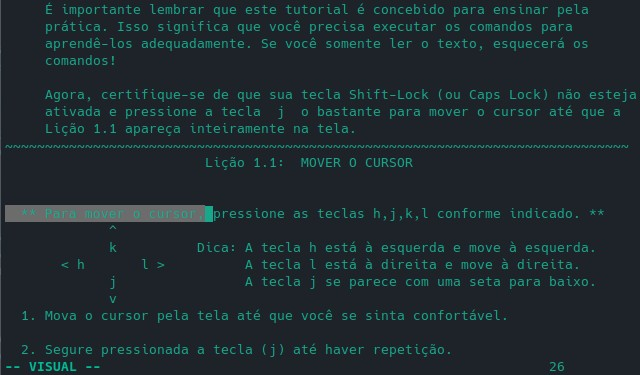
\includegraphics[scale=0.5]{introducao/modo_visual.jpg}
%\label{introducao_005}
\caption{Modo visual em ação.}
\end{figure}

\subsubsection{Modo Visual Linha}
Neste, a seleção muda de lógica.
É muito eficiente para a seleção de trechos maiores.
Parágrafos, trechos de centenas de linhas, basta selecionar e então realizar sua ação.

\begin{figure}[!htb]
\centering
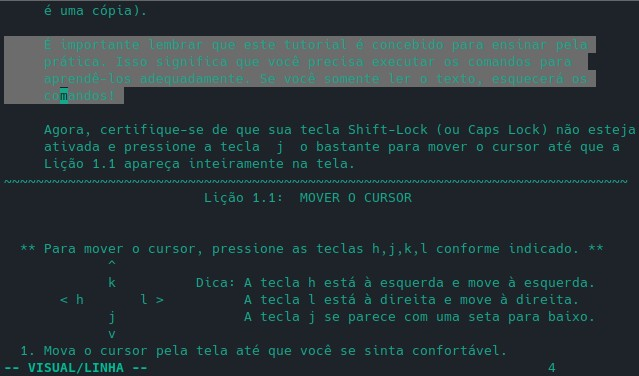
\includegraphics[scale=0.5]{introducao/modo_visual_linha.jpg}
%\label{introducao_006}
\caption{Modo visual-linha em ação.}
\end{figure}

Destrua, reconstrua, altere ou defina um escopo para aplicar suas mudanças.
Para entrar neste modo, \vimcommand{V}, maiúsculo.

\subsubsection{Modo Visual Bloco}
A última variação do modo visual seleciona baseado em colunas.
Seu foco é a alteração de texto tabelado.
Também é interessante para a seleção vertical no geral, como em blocos de código que estão indentados.

Tudo o mais também é válido, seja salvar, recortar, ou usar como escopo para ações.
Para entrar neste modo, \vimcommand{CTRL-v}.

\begin{figure}[!htb]
\centering
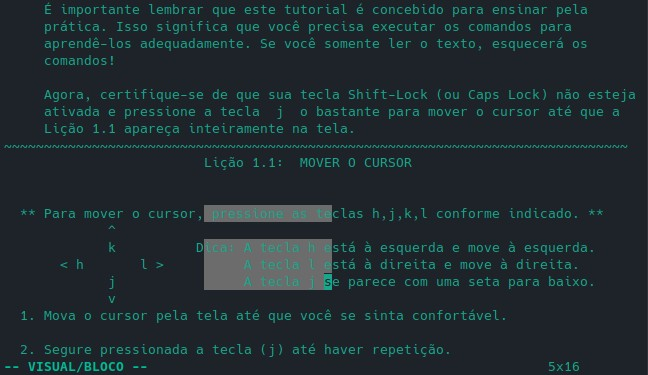
\includegraphics[scale=0.5]{introducao/modo_visual_bloco.jpg}
%\label{introducao_007}
\caption{Modo visual-bloco em ação.}
\end{figure}

\subsection{Marks}
Esse tópico se confunde com outro, referente ao modelo de memória que o vim usa para armazenar diferentes tipos de dados.
Sempre que você realiza um salto, você deixa um rastro.
Mas e se você quiser armazenar uma posição para onde você pode voltar?

Futuramente vamos poder explorar a edição de múltiplos arquivos.
Imagine o potencial de deixar uma pequena marca em uma parte específica de um arquivo,
então digitar uma sequência de teclas, e o editor simplesmente te deixar onde você pode continuar o trabalho.
São saltos avançados.

Para definir uma marca, utilize o comando \vimcommand{:ma [caractere]}, e uma marca será definida na posição do cursor.
Para ir até a marca existem duas maneiras.
A primeira é utilizando o caractere crase \vimcommand{\`}\vimcommand{a}.
A segunda é utilizando aspas simples. \vimcommand{'}\vimcommand{a}.

O vim define marcas para todo tipo de coisa, seja qual foi sua última alteração de texto,
qual foi a última vez que entrou no modo de edição,
e até mesmo qual foi o último trecho que foi selecionado dentro do modo visual.

Para verificar quais os marks definidos, use \vimcommand{:marks}. Perceba quais são os caracteres utilizados para armazená-los.

Como existem muitos detalhes, e não é tudo que é interessante, fica como atividade para o leitor explorar no manual mais tarde.
Mas para completar a explicação, existem marcas salvas nos caracteres a-z, 
que são salvas referentes ao arquivo atual, e marcas salvas nos caracteres A-Z,
que salvam também o nome e caminho do arquivo.
Alguns caracteres são de uso automático, então ele provavelmente será sobrescrito, mas para saber quais são, leia o manual.

\begin{figure}[!htb]
\centering
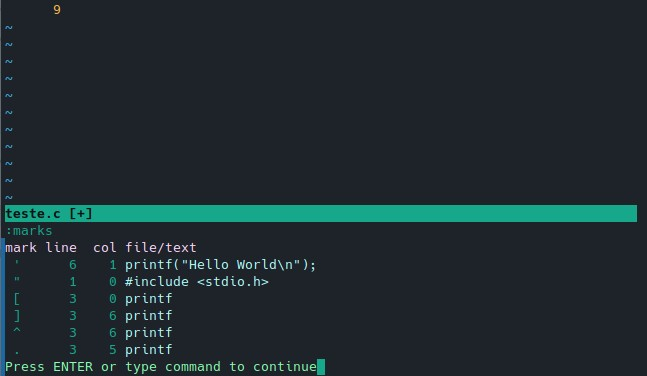
\includegraphics[scale=0.8]{introducao/marks_exemplo.jpg}
%\label{introducao_008}
\caption{Lista de marks.}
\end{figure}

\newpage
